\section{Numerical Experiments}
\label{sec:experiments}

\In this section, we present a comprehensive evaluation of our Nested WAIT algorithm through numerical experiments. Our analysis focuses on a real-world dataset sourced from \cite{zheng2023lmsys} to assess its performance in practical settings. All experiments are conducted using Microsoft Vidur to simulate an NVIDIA A100 GPU, mirroring the hardware configuration employed in prior studies \citep{agrawal2024vidur}. We benchmark our WAIT algorithm against vLLM \citep{kwon2023efficient} and Sarathi \citep{agrawal2023sarathi}, widely recognized inference engines that employ First-Come-First-Serve (FCFS) scheduling. Specifically, vLLM prioritizes new arrivals, while Sarathi prioritizes ongoing prompts, with both enforcing fixed limits on the total number of tokens and prompts per iteration.

To start with, we evaluate the Nested WAIT algorithm, designed for scenarios where prompt output lengths are unknown. We test it on both synthetic and real-world datasets, using the same batch size limits across all algorithms and setting thresholds proportional to arrival rates in each segment for practical implementation.

We begin with a synthetic dataset where \( m=4 \), prefill lengths are fixed at 10 tokens, decode lengths are \( (20, 40, 80, 160) \), and arrival rates follow a \( 20:40:80:160 \) ratio. We set thresholds \( (n_1, n_2, n_3, n_4) \) with the ratio \( 15:14:12:8 \). Figure \ref{fig:comparison Nested WAIT, short prefill} shows improved throughput and latency over benchmarks.

For real-world testing, we use the dataset from \cite{zheng2023lmsys}, which contains over 210,000 prompts from Vicuna and Chatbot Arena. We treat questions as prompts and answers as decoded tokens. Figure \ref{fig:distribution} shows the distribution of prefill and decode lengths. We randomly sample 50,000 prompts and simulate arrivals via a Poisson process.

To implement Nested WAIT, we group decode lengths (1 to 500 tokens) into 10 bins of 50 tokens each (e.g., [1-50], [51-100], etc). For each bin, we compute the mean prefill length (approximately 60 tokens, as shown in Figure \ref{fig:group}) and arrival rates proportional to \( 23:11:8:7:6:4:3:2:1:1 \). We set \( m=10 \) and thresholds \( (n_1, \dots, n_{10}) \) with the ratio \( 66:43:32:24:17:11:7:4:2:1 \), following \eqref{eq:nested_wait_thresholds}. Prompts in the \( k \)-th decode stage are assigned to segment \( \lceil k/50 \rceil \).
% More discussions on this segment design are left in Appendix \ref{sec:extension}.

We first test a synthetic workload with prefill fixed at 60 tokens and decode lengths clustered into 10 types (50, 100, ..., 500 tokens), with arrival rates matching the real dataset's proportions. We evaluate Nested WAIT with queries per second (QPS) of 55 and 550, shown in Figure \ref{fig:comparison_Nested_WAIT_real_world_low} and Figure \ref{fig:comparison Nested WAIT, real world, higher rate}, respectively. Nested WAIT outperforms benchmarks in both throughput and latency.

% \gan{Maybe, we can say that the Figure \ref{fig:comparison_Nested_WAIT_real_world_low} and Figure \ref{fig:comparison Nested WAIT, real world, higher rate} are on static arrival rate, and Figure \ref{fig:comparison Nested WAIT, real world} is on time-varying arrival rate bt with static threshold, which leads to a little latency overflow.}

Finally, we test the real dataset with original prefill and decode lengths, using the same thresholds. Figure \ref{fig:comparison Nested WAIT, real world} shows that Nested WAIT achieves higher throughput with a modest increase in latency (approximately 0.5 seconds per prompt), enhancing system efficiency while maintaining responsiveness. The designed thresholds are on time-varying arrival rate but with static threshold, which leads to a little bit more latency.

\begin{figure}[ht]
    \centering
    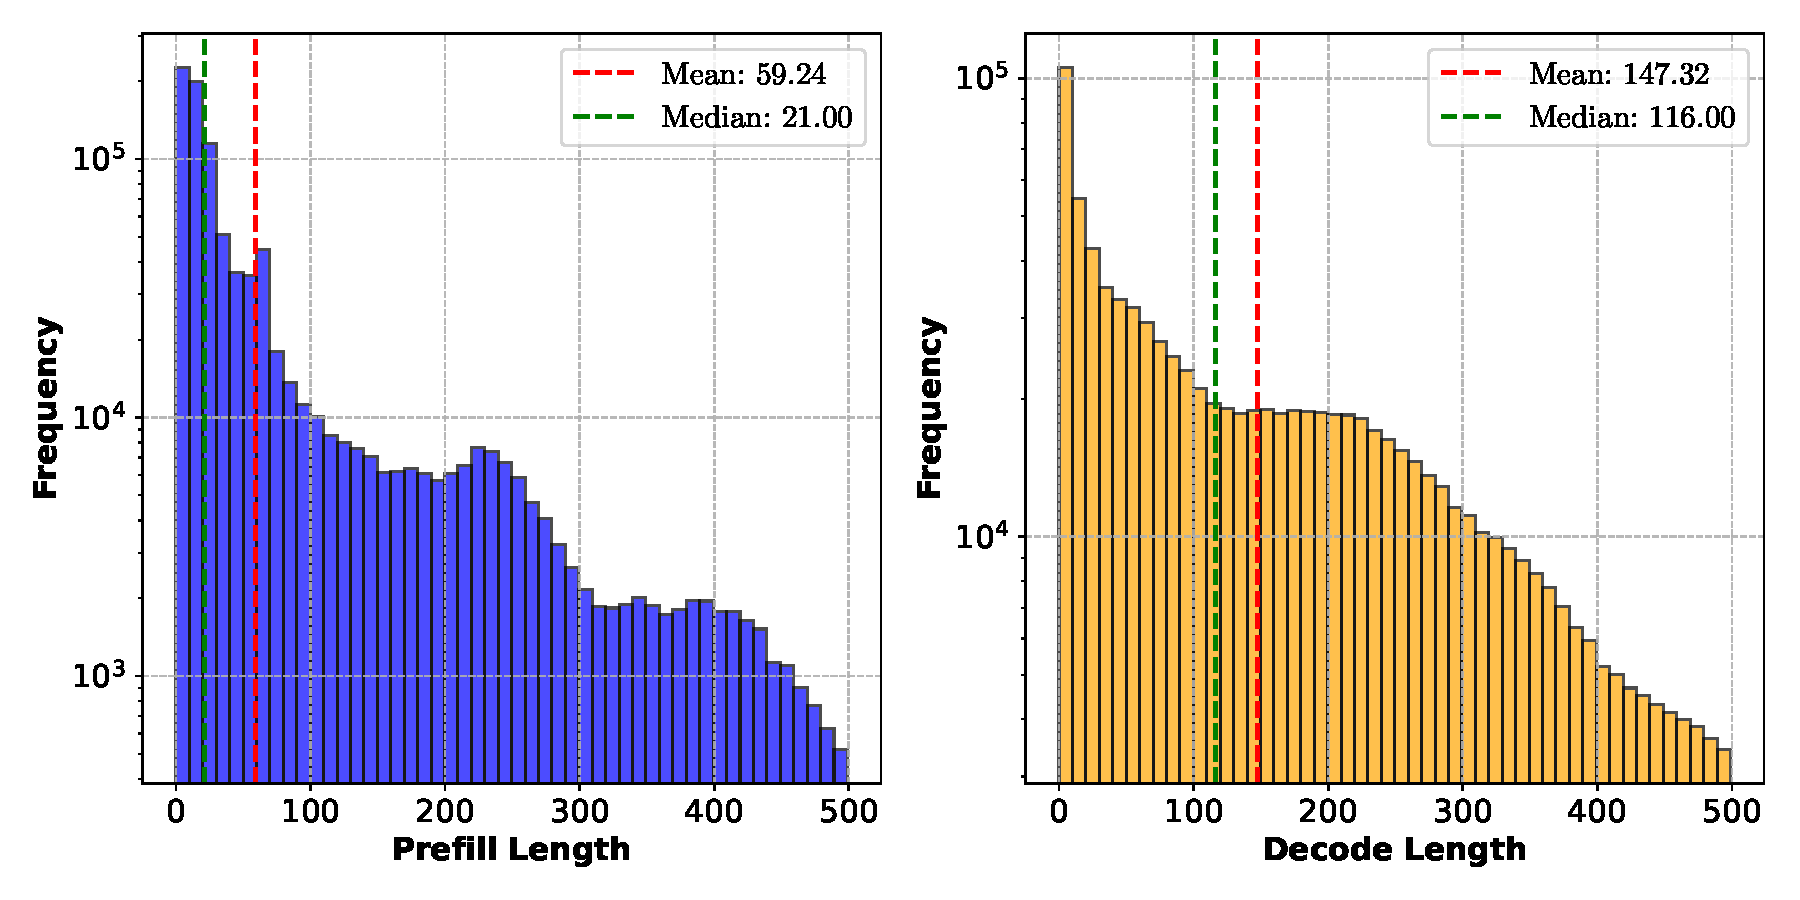
\includegraphics[width=0.6\textwidth]{Experiments_pdf/question_answer_lengths_distribution.pdf}
    \caption{Distribution of prefill and decode lengths in the real dataset.}
    \label{fig:distribution}
\end{figure}

\begin{figure}[ht]
    \centering
    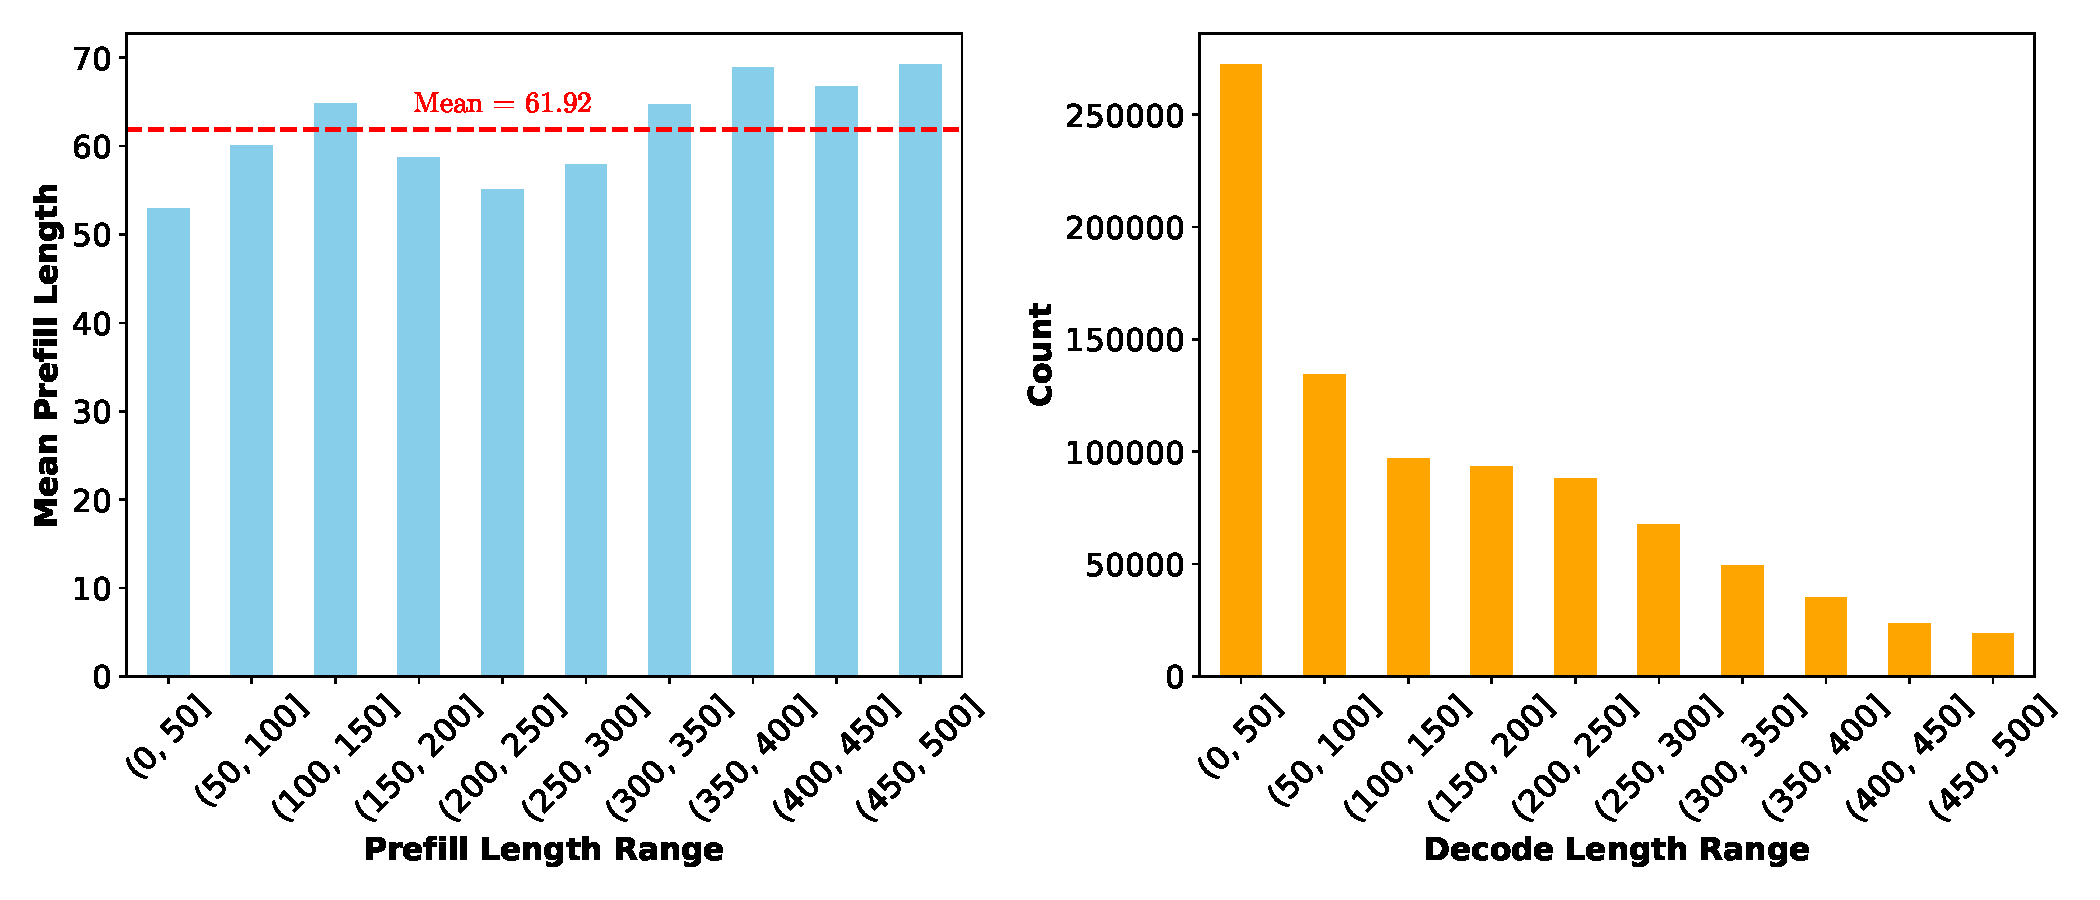
\includegraphics[width=0.6\textwidth]{Experiments_pdf/group.pdf}
    \caption{Mean prefill lengths and prompt counts per decode length bin in the real dataset.}
    \label{fig:group}
\end{figure}

\begin{figure}[htbp]
    \centering
    \begin{minipage}{0.4\textwidth}
        \centering
        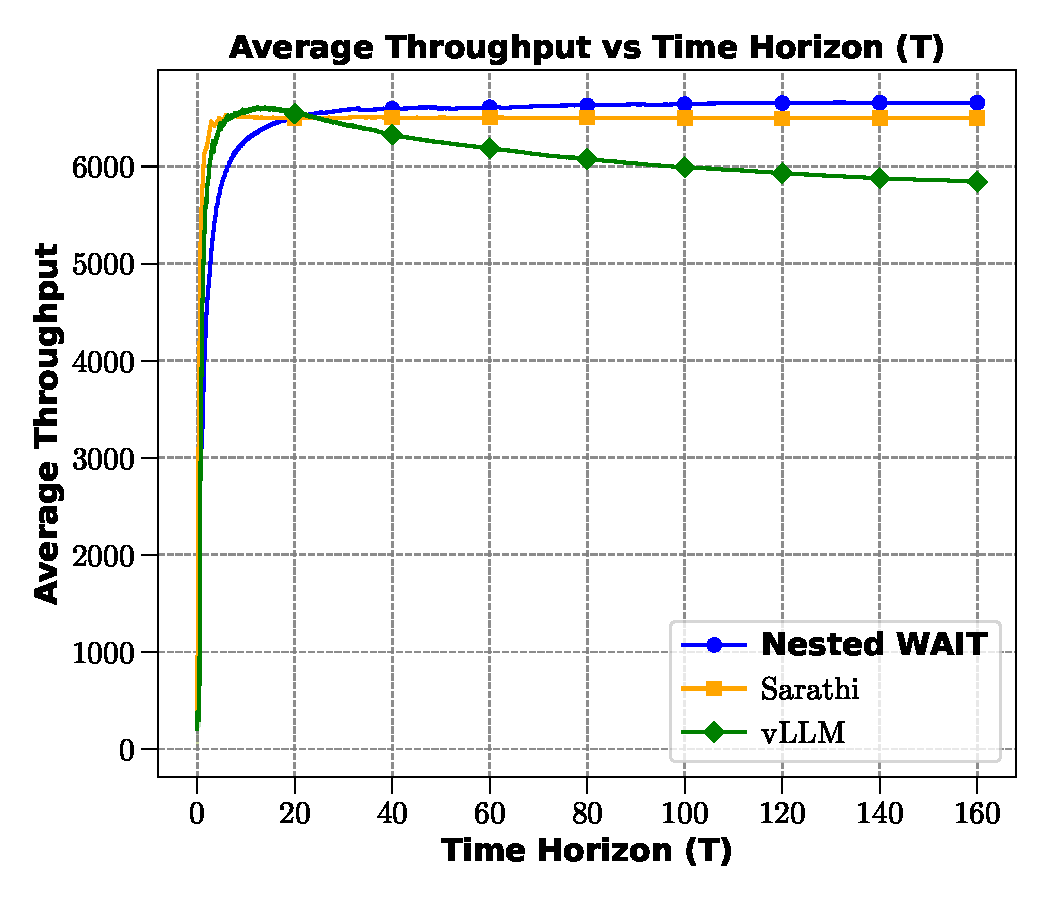
\includegraphics[width=\textwidth]{Experiments_pdf/test30_simulated_short_decode_bs=128_nested_real_not_trace_throughput.pdf}
    \end{minipage}
    \hfill
    \begin{minipage}{0.4\textwidth}
        \centering
        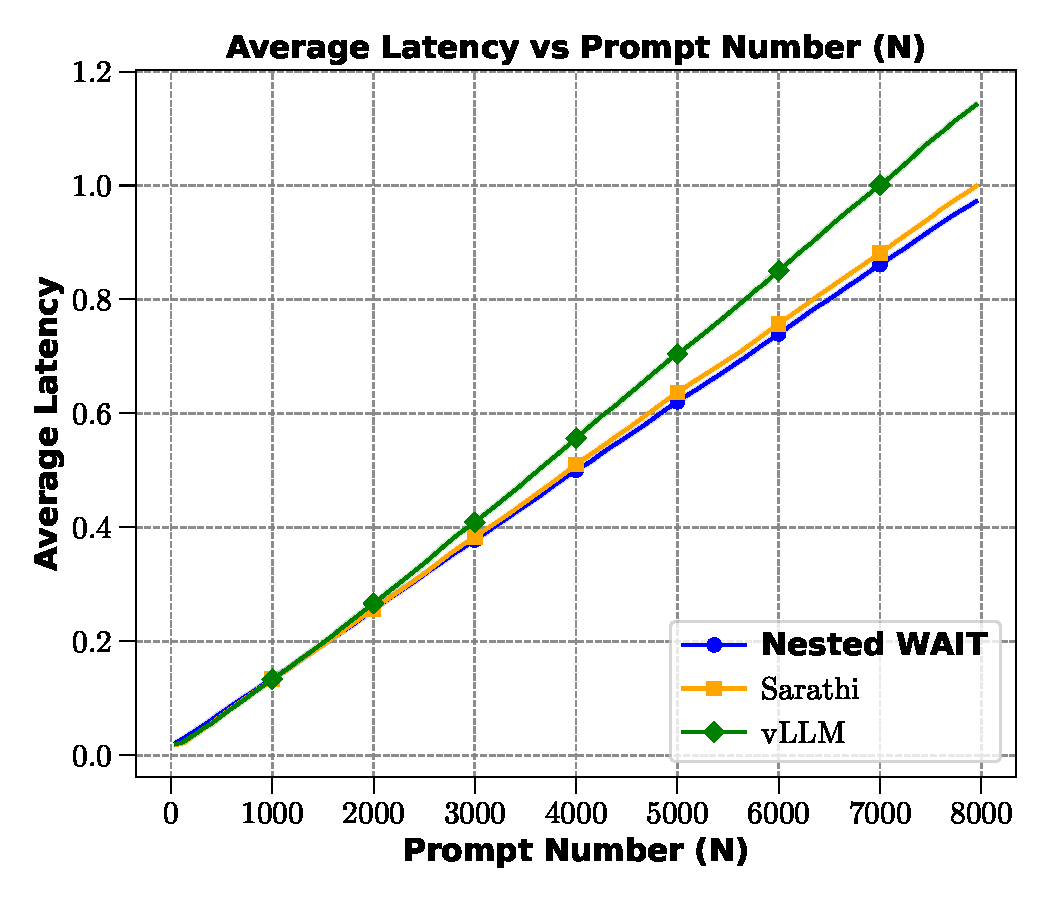
\includegraphics[width=\textwidth]{Experiments_pdf/test30_simulated_short_decode_bs=128_nested_real_not_trace_latency.pdf}
    \end{minipage}
    \caption{Average throughput and latency across algorithms on the synthetic dataset.}
    \label{fig:comparison Nested WAIT, short prefill}
\end{figure}

\begin{figure}[htbp]
    \centering
    \begin{minipage}{0.4\textwidth}
        \centering
        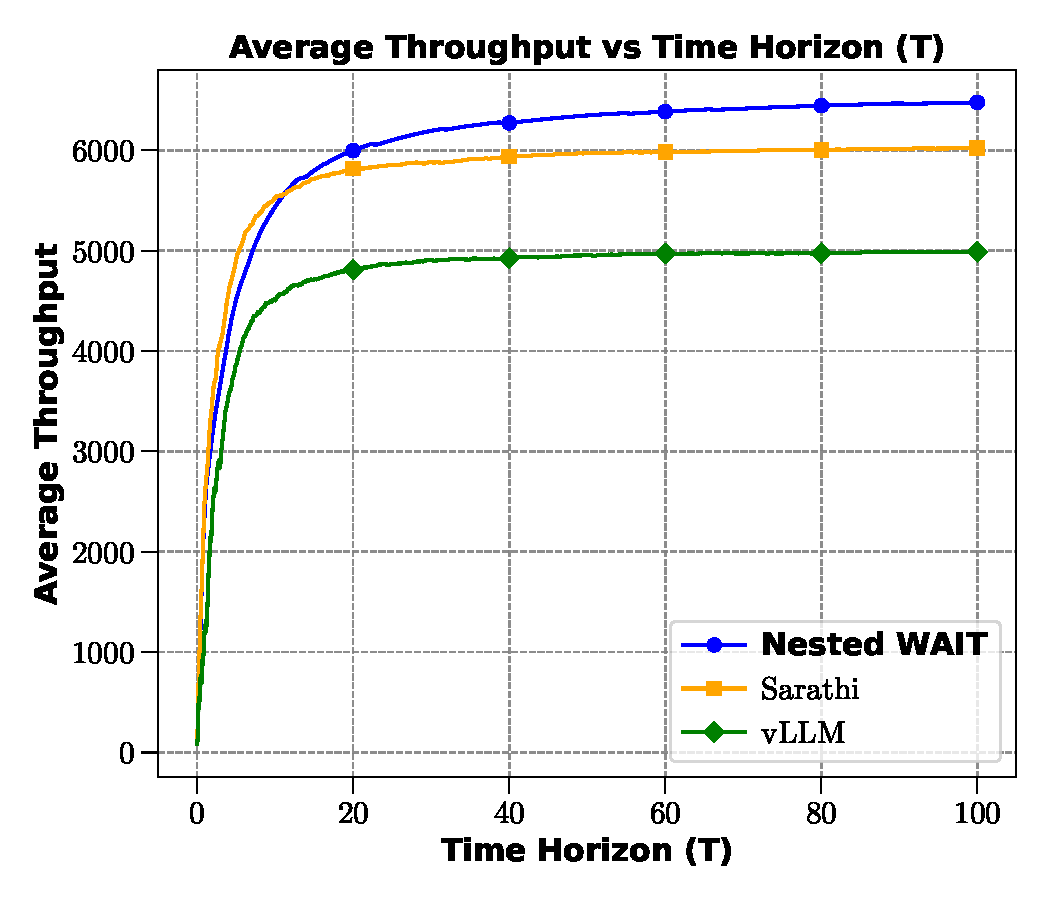
\includegraphics[width=\textwidth]{Experiments_pdf/test31_simulated_short_decode_bs=148_nested_real_not_trace_throughput.pdf}
    \end{minipage}
    \hfill
    \begin{minipage}{0.4\textwidth}
        \centering
        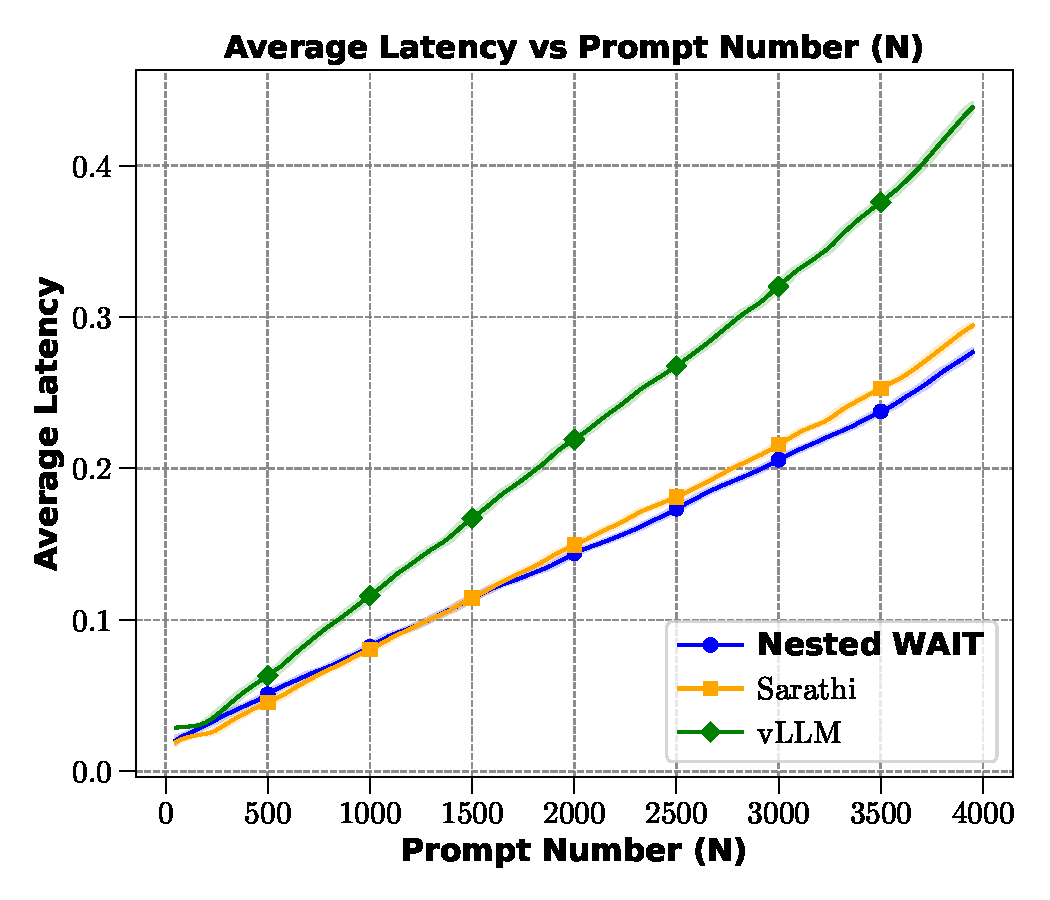
\includegraphics[width=\textwidth]{Experiments_pdf/test31_simulated_short_decode_bs=148_nested_real_not_trace_latency.pdf}
    \end{minipage}
    \caption{Average throughput and latency across algorithms on the real dataset with clustered output lengths (low arrival rates).}
    \label{fig:comparison_Nested_WAIT_real_world_low}
\end{figure}

\begin{figure}[htbp]
    \centering
    \begin{minipage}{0.4\textwidth}
        \centering
        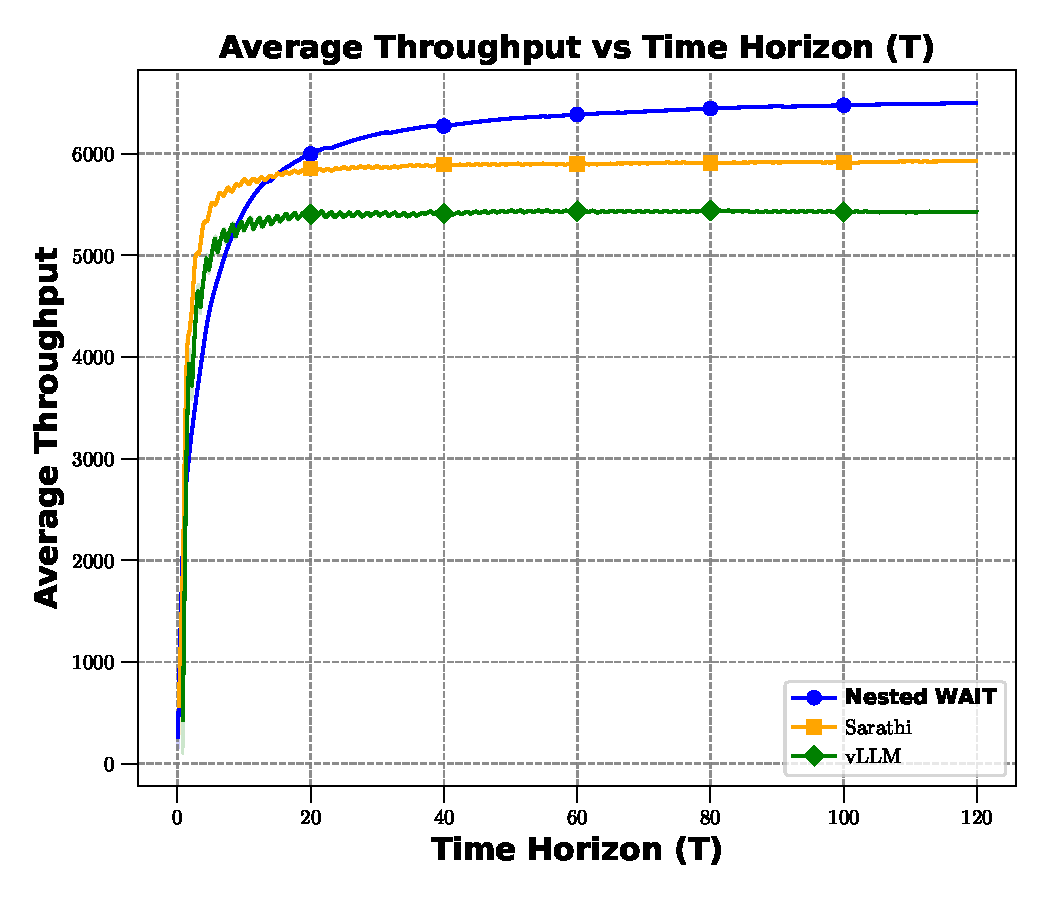
\includegraphics[width=\textwidth]{Experiments_pdf/test32_simulated_short_decode_bs=148_nested_real_not_trace_higher_rate_throughput.pdf}
    \end{minipage}
    \hfill
    \begin{minipage}{0.4\textwidth}
        \centering
        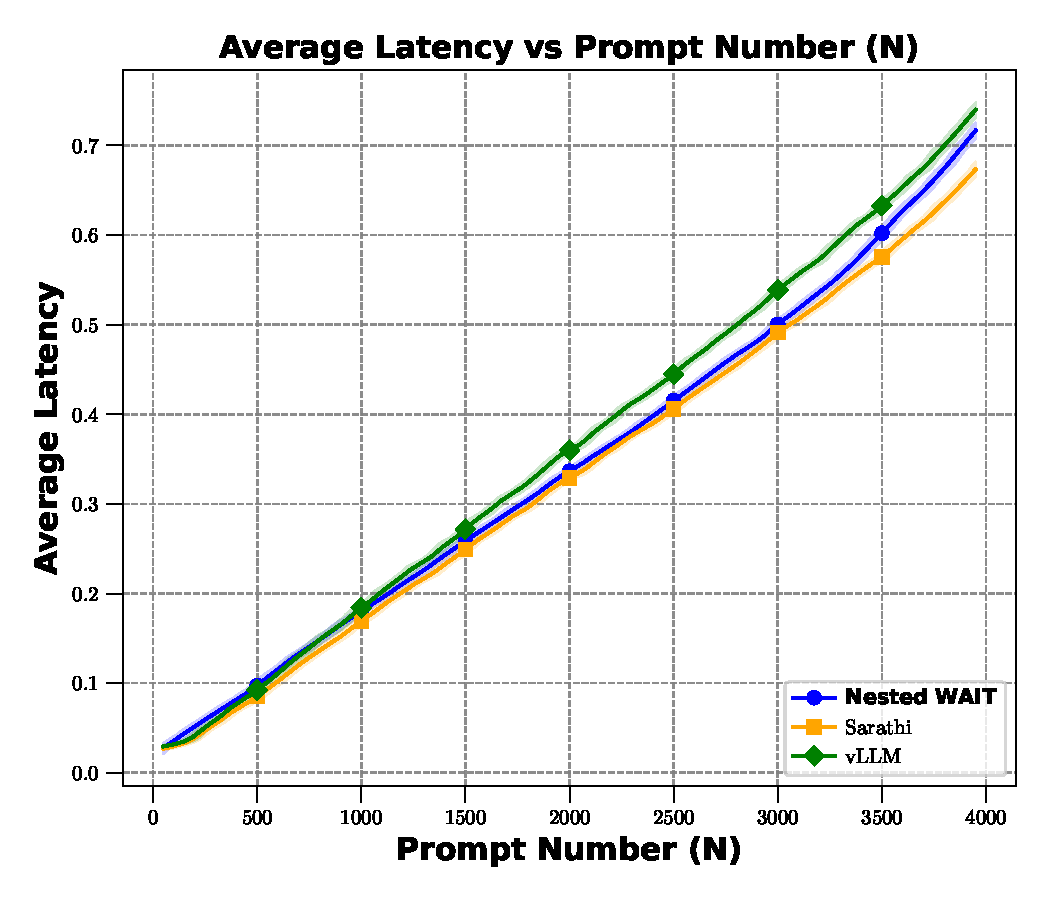
\includegraphics[width=\textwidth]{Experiments_pdf/test32_simulated_short_decode_bs=148_nested_real_not_trace_higher_rate_latency.pdf}
    \end{minipage}
    \caption{Average throughput and latency across algorithms on the real dataset with clustered output lengths (high arrival rates).}
    \label{fig:comparison Nested WAIT, real world, higher rate}
\end{figure}

\begin{figure}[htbp]
    \centering
    \begin{minipage}{0.4\textwidth}
        \centering
        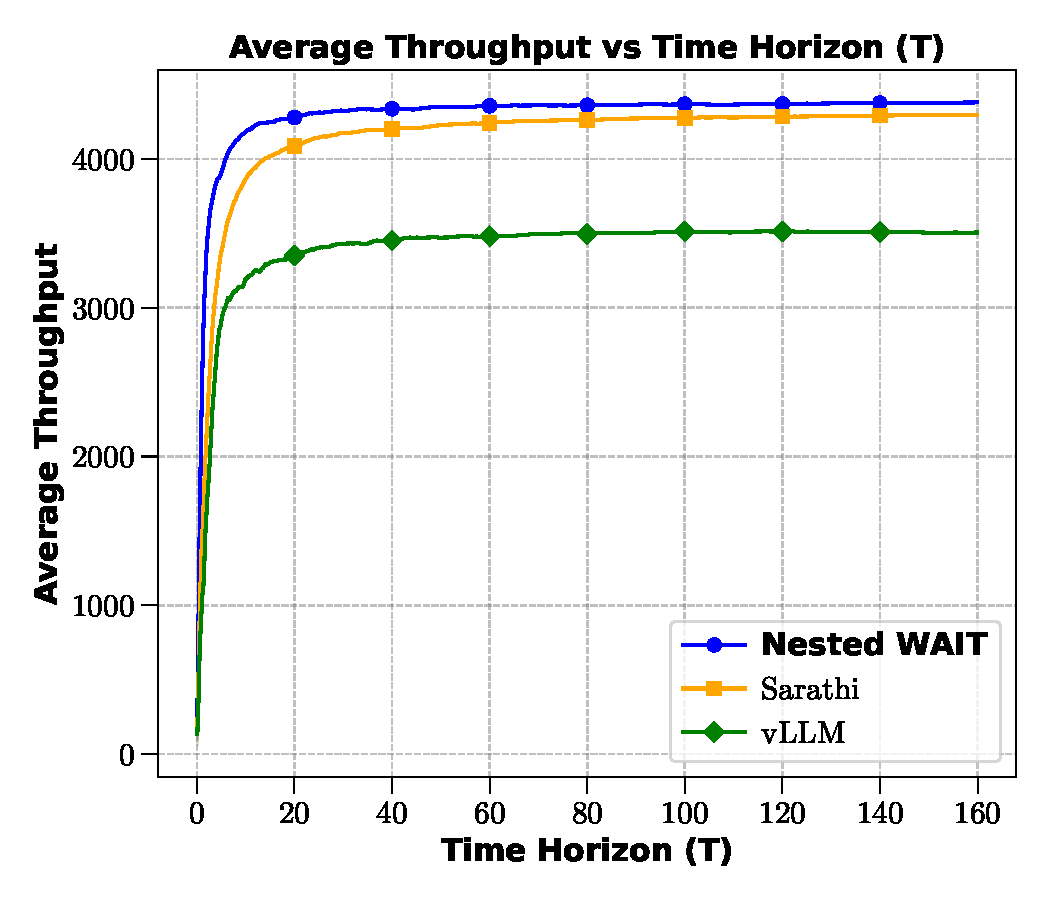
\includegraphics[width=\textwidth]{Experiments_pdf/test36_simulated_short_decode_bs=64_nested_real_TRACE_throughput.pdf}
    \end{minipage}
    \hfill
    \begin{minipage}{0.4\textwidth}
        \centering
        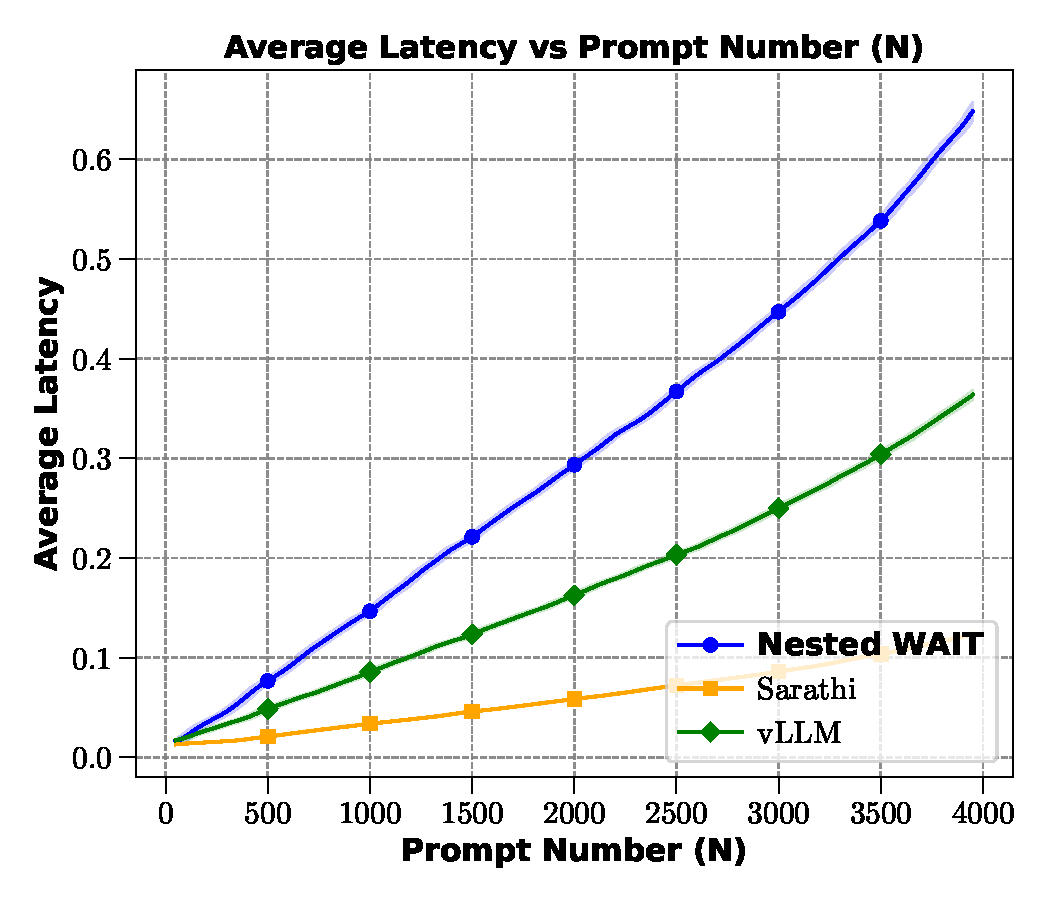
\includegraphics[width=\textwidth]{Experiments_pdf/test36_simulated_short_decode_bs=64_nested_real_TRACE_latency.pdf}
    \end{minipage}
    \caption{Average throughput and latency across algorithms on the real dataset with actual output lengths.}
    \label{fig:comparison Nested WAIT, real world}
\end{figure}